% =========================================================================
% Capítulo 2: Cinética de la partícula
% Tema 01: Dinámica de la partícula
% Problema 04: Anillo en aro circular con resorte
% =========================================================================
\subsubsection{Anillo en aro circular con resorte}

Un anillo de masa $m$ se encuentra inserto en un aro circular vertical de radio $R$ y centro $O$. El aro está soldado, en su punto $A$, a una barra horizontal de largo $R$ que lo hace girar con velocidad angular constante $\Omega_0$ respecto a un eje vertical (el centro del aro queda entonces a una distancia $2R$ del eje). Un resorte ideal de constante elástica $k$ y longitud natural $\ell_0$ une, siguiendo la trayectoria del aro, al anillo con el punto $A$. La posición del anillo $P$ se mide con el ángulo $\varphi$ desde la recta $OA$, como se muestra en la Figura \ref{fig:anillo_aro}. Realice lo siguiente:

\begin{enumerate}
    \item Defina los marcos de referencia y los sistemas de coordenadas adecuados para describir el movimiento del anillo en el espacio.
    \item Determine el vector posición del anillo respecto al punto $S$ del eje de giro que está a la altura de $O$, en términos del ángulo $\varphi$.
    \item Obtenga los vectores de velocidad angular y aceleración angular del aro respecto al suelo.
    \item Calcule los vectores de velocidad y aceleración del anillo vistos por un observador fijo al suelo.
    \item Determine la ecuación diferencial del movimiento del anillo en términos de $\varphi$.
\end{enumerate}

\begin{figure}[!ht]
    \centering
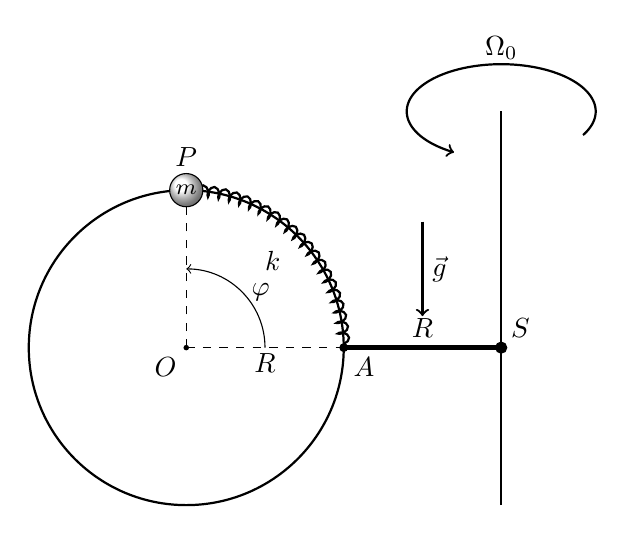
\begin{tikzpicture}[scale=2]
  % Radius
  \def\R{1}

  \coordinate (O) at (0,0);
  \coordinate (A) at (0,\R);
  \coordinate (P) at (\R,0);

  % Circle
  \draw[thick] (0,0) circle(\R);

  % Axes / radius lines
  \draw[dashed] (0,0) -- (0,\R);          % OA
  \draw[dashed] (0,0) -- (\R,0);          % OP

  % Points
  \fill (0,0) circle (0.5pt) node[below left] {$O$};
  \fill (0,\R) circle (1pt) node[above=5pt] {$P$};
 
  \fill (\R,0) circle (0.8pt) node[below right] {$A$};
  
        \draw[->] (0.5, 0) arc (0:90:0.5) node[midway, right] {$\varphi$};

  % Radius label
  \node at (0.5,-0.1) {$R$};
  \node[above] at (1.5*\R,0) {$R$};
  \filldraw (2*\R,0) circle (1pt) node[above right] {$S$};

  % Spring along arc from A to P (quarter circle, clockwise)
  \draw[decoration={coil, aspect=0.5, segment length=4pt, amplitude=2pt},
        decorate, thick] 
        (0,\R) arc[start angle=90, end angle=0, radius=\R];

  % Label for spring constant
  \node at (0.55,0.55) {$k$};

  
 \shadedraw[ball color=white] (0, \R) circle (3pt) node[font=\footnotesize] {$m$};
  % Horizontal bar from P to O (thick)
  \draw[line width=2pt] (\R,0) -- (2*\R,0);

  % Gravity vector
  \draw[->, thick] (1.5*\R,0.8) -- ++(0,-0.6);
  \node[right] at (1.5*\R,0.5) {$\vec{g}$};


 \draw[-,thick] (2,-1)--(2,1.5); 
    \begin{scope}[shift={(2,1.5)}, rotate=0]
    \draw[->,thick] 
      plot[domain=-30:240,variable=\t,smooth,samples=100] 
      ({0.6*cos(\t)}, {0.3*sin(\t)});
    \node at (0,0.4) {$\Omega_0$};
  \end{scope}

\end{tikzpicture}
    \caption{Sistema de anillo sobre aro circular giratorio con vínculo elástico.}
    \label{fig:anillo_aro}
\end{figure}

% --- SOLUCIÓN ---------------------------------------------------------------
\begin{solucion}{Anillo en aro circular con resorte}

\textbf{Marcos de referencia y Sistemas de Coordenadas}
\begin{itemize}
    \item $\mathcal{N}$: suelo (inercial) $\longrightarrow\{\vec{e}_x;\vec{e}_y;\vec{e}_z\}$, con origen en $S$ (punto del eje de giro a la altura de $O$).
    \item $\mathcal{A}$: aro $\longrightarrow\{\vec{e}_r;\vec{e}_\theta;\vec{e}_z\}$ (cilíndrica fija en el aro, con $\vec{e}_r$ horizontal desde el eje hacia el centro del aro).
    \item $\mathcal{B}$: marco imaginario orientado desde $O$ (centro del aro) hacia el anillo $P$ $\longrightarrow\{\vec{E}_r;\vec{E}_\varphi;\vec{e}_\theta\}$ en el plano del aro.
\end{itemize}

\begin{center}
\begin{tikzpicture}[>=Latex, scale=1.3]
    % --- PARÁMETROS ---
    \def\R{1.6}     % radio del aro [u]
    \def\ph{50}     % ángulo varphi [°]

    % --- EJE Y BARRA ---
    \draw[thick] (0,-1.5*\R) -- (0,1.7*\R);
    \draw[->, thick] (0,1.5*\R) -- (0,1.7*\R) node[above] {$\Omega_0$};
    \draw[line width=2pt] (0,0) -- (\R,0);
    \filldraw (0,0) circle (1.2pt) node[below left] {$S$};

    % --- ARO ---
    \coordinate (C) at (2*\R,0);
    \coordinate (A) at (\R,0);
    \coordinate (M) at ({2*\R-\R*cos(\ph)},{\R*sin(\ph)});
    \draw[thick] (C) circle (\R);
    \draw[dashed, gray] (C) -- (A);
    \draw[decoration={coil, aspect=0.5, segment length=3pt, amplitude=1.6pt}, decorate, thick]
        (A) arc (180:{180-\ph}:\R);
    \filldraw (C) circle (1pt) node[below right] {$O$};
    \filldraw (A) circle (1.2pt) node[below left] {$A$};
    \shadedraw[ball color=gray!30] (M) circle (3.5pt) node[above left] {$P$};

    % --- BASES ---
    \draw[azul, ultra thick, -{Latex}] (C) -- ++(0.9,0) node[right] {$\vec{e}_r$};
    \draw[azul, ultra thick, -{Latex}] (C) -- ++(0,0.9) node[right] {$\vec{e}_z$};
    \draw[myred, ultra thick, -{Latex}] (C) -- ({2*\R-0.9*cos(\ph)},{0.9*sin(\ph)}) node[below left, xshift=1pt, yshift=2pt] {$\vec{E}_r$};
    \draw[myred, ultra thick, -{Latex}] (M) -- ++({90-\ph}:0.9) node[above right] {$\vec{E}_\varphi$};
    \draw[->] ($(C)+(180:0.5)$) arc (180:{180-\ph}:0.5);
    \node at ({2*\R-0.75*cos(\ph/2)},{0.75*sin(\ph/2)-0.05}) {$\varphi$};
\end{tikzpicture}
\end{center}

\begin{equation*}
\begin{split}
    \vec{e}_r&=\cos(\Omega_0 t)\vec{e}_x+\sin(\Omega_0 t)\vec{e}_y\\
    \vec{e}_\theta&=-\sin(\Omega_0 t)\vec{e}_x+\cos(\Omega_0 t)\vec{e}_y\\
    \vec{E}_r&=-\cos\varphi\,\vec{e}_r+\sin\varphi\,\vec{e}_z\\
    \vec{E}_\varphi&=\sin\varphi\,\vec{e}_r+\cos\varphi\,\vec{e}_z
\end{split}
\end{equation*}

\textbf{Velocidad angular del aro}\\
$$\velang{N}{A}=\Omega_0\vec{e}_z\qquad\accang{N}{A}=\vec{0}$$

\subsubsection*{Cinemática de la partícula}
\textbf{Posición}\\
Como siempre, para obtener la velocidad respecto a un marco inercial partimos de la posición del anillo, medida desde un punto que no se mueve ($S$):
\begin{align*}
    \vec{r}_P &= 2R\,\vec{e}_r + R\,\vec{E}_r \\
              &= 2R\,\vec{e}_r + R\left[ -\cos\varphi\,\vec{e}_r + \sin\varphi\,\vec{e}_z \right] \\
              &= R\left(2 - \cos\varphi\right)\vec{e}_r + R\sin\varphi\,\vec{e}_z
\end{align*}

\textbf{Velocidad}\\
La velocidad es la derivada temporal de la posición:
\begin{align*}
\der{\vec{r}_P}{N}{} &= R \sin\varphi\,\dot{\varphi}\,\vec{e}_r + R(2 - \cos\varphi)\der{\vec{e}_r}{N}{} + R \cos\varphi\,\dot{\varphi}\,\vec{e}_z
\end{align*}

\patotruco{Aquí no hace falta escribir el teorema del transporte completo: como $\vec{e}_r$ y $\vec{e}_\theta$ solo giran en torno a $\vec{e}_z$ con velocidad angular $\Omega_0$, el trucazo es derivar $\vec{e}_r\to\Omega_0\vec{e}_\theta$ y $\vec{e}_\theta\to-\Omega_0\vec{e}_r$ (la demostración está en la Ayudantía 5).}

Derivadas temporales de $\vec{e}_r$ y $\vec{e}_\theta$:
$$\transport{\vec{e}_r}{N}{A}=\Omega_0\vec{e}_z\times\vec{e}_r=\Omega_0\vec{e}_\theta$$
$$\transport{\vec{e}_\theta}{N}{A}=\Omega_0\vec{e}_z\times\vec{e}_\theta=-\Omega_0\vec{e}_r$$
y finalmente
$$\marc{\vec{v}_P}{N}= R \sin\varphi\,\dot{\varphi}\,\vec{e}_r + R(2 - \cos\varphi)\,\Omega_0\,\vec{e}_\theta + R \cos\varphi\,\dot{\varphi}\,\vec{e}_z$$

\textbf{Aceleración}\\
Al igual que antes, derivamos la velocidad:
\begin{align*}
\marc{\vec{a}_P}{N}=\der{\vec{v}_P}{N}{} &= R \left[
\left( \ddot{\varphi} \sin\varphi + \dot{\varphi}^2 \cos\varphi - (2 - \cos\varphi) \Omega_0^2 \right) \vec{e}_r \right. \\
&\quad + \left(2 \dot{\varphi} \sin\varphi\, \Omega_0 \right) \vec{e}_\theta \\
&\quad + \left. \left( \ddot{\varphi} \cos\varphi - \dot{\varphi}^2 \sin\varphi \right) \vec{e}_z \right]
\end{align*}

\subsubsection*{Cinética}
\textbf{Diagrama de cuerpo libre}\\
Siempre se parte por un DCL, vista del plano $\vec{e}_r$-$\vec{e}_z$ (la normal $\vec{N}_\theta$ sale del plano):
\begin{center}
\begin{tikzpicture}[>=Latex, scale=1.0]
    \def\ph{50}
    \coordinate (M) at (0,0);
    \draw[->, thick, myred] (M) -- ++({180-\ph}:1.3) node[above left] {$\vec{N}_r$};
    \draw[->, thick, myred] (M) -- ++({270-\ph}:1.1) node[below left] {$\vec{F}_s$};
    \draw[->, thick, myred] (M) -- ++(0,-1.2) node[below] {$\vec{F}_g$};
    \shadedraw[ball color=gray!30] (M) circle (4pt);
    \node[above right] at (M) {$m$};
    \node at (1.3,0.9) {$\vec{N}_\theta$};
    \draw (1.8,0.9) circle (0.12); \fill (1.8,0.9) circle (1pt);
\end{tikzpicture}
\end{center}

Después del DCL se caracteriza cada fuerza vectorialmente. La fuerza de un resorte curvo tiene la dirección tangente de la curva en la que está contenido, en este caso $\vec{E}_\varphi$:
$$\vec{F}_s=-k(\ell-\ell_0)\vec{e}_t=-k(R\varphi-\ell_0)\vec{E}_{\varphi}=-k(R\varphi-\ell_0)\left(\sin\varphi\,\vec{e}_r+\cos\varphi\,\vec{e}_z\right)$$
$$\vec{F}_g=-mg\,\vec{e}_z$$
Al igual que en otros problemas, las direcciones de las normales son las direcciones normal y binormal de la curva:
$$\vec{N}_r=N_r\vec{E}_r=N_r\left( -\cos\varphi\,\vec{e}_r + \sin\varphi\,\vec{e}_z \right)$$
$$\vec{N}_\theta=N_\theta\vec{e}_\theta$$

\patoojo{El resorte curvo no tira en línea recta hacia $A$: su fuerza es tangente al aro y su largo es el arco $\ell=R\varphi$ (no la cuerda).}

\textbf{Ecuación diferencial}\\
Se plantea la segunda ley de Newton $\sum\vec{F}_{ext}=m\marc{\vec{a}_P}{N}$, proyectada en $\vec{e}_r$, $\vec{e}_\theta$ y $\vec{e}_z$:
\begin{align*}
-k(R\varphi-\ell_0)\sin\varphi - N_r\cos\varphi &= Rm \left( \ddot{\varphi} \sin\varphi + \dot{\varphi}^2 \cos\varphi - (2 - \cos\varphi) \Omega_0^2 \right)\\
N_\theta &= Rm \cdot 2 \dot{\varphi} \sin\varphi\, \Omega_0 \\
N_r\sin\varphi - mg - k(R\varphi - \ell_0)\cos\varphi &= Rm \left( \ddot{\varphi} \cos\varphi - \dot{\varphi}^2 \sin\varphi \right)
\end{align*}
Ignoramos la segunda ecuación, ya que no contiene $\ddot{\varphi}$.

\textbf{Paso 1: despejar $N_r$ de la primera ecuación.}
$$N_r = \frac{ -Rm \left( \ddot{\varphi} \sin\varphi + \dot{\varphi}^2 \cos\varphi - (2 - \cos\varphi) \Omega_0^2 \right) - k(R\varphi - \ell_0)\sin\varphi }{ \cos\varphi }$$

\textbf{Paso 2: sustituir $N_r$ en la tercera ecuación.}
\begin{multline*}
\left( \frac{ -Rm \left( \ddot{\varphi} \sin\varphi + \dot{\varphi}^2 \cos\varphi - (2 - \cos\varphi) \Omega_0^2 \right) - k(R\varphi - \ell_0)\sin\varphi }{ \cos\varphi } \right)\sin\varphi\\
- mg - k(R\varphi - \ell_0)\cos\varphi = Rm \left( \ddot{\varphi} \cos\varphi - \dot{\varphi}^2 \sin\varphi \right)
\end{multline*}

\textbf{Paso 3: expandir el lado izquierdo.}
\begin{multline*}
\frac{ -Rm \ddot{\varphi} \sin^2\varphi - Rm \dot{\varphi}^2 \cos\varphi\sin\varphi + Rm(2 - \cos\varphi) \Omega_0^2 \sin\varphi - k(R\varphi - \ell_0)\sin^2\varphi }{\cos\varphi}\\
- mg - k(R\varphi - \ell_0)\cos\varphi = Rm \ddot{\varphi} \cos\varphi - Rm \dot{\varphi}^2 \sin\varphi
\end{multline*}

\textbf{Paso 4: agrupar los términos con $\ddot{\varphi}$.}
$$\ddot{\varphi} \left( -Rm \left( \frac{\sin^2\varphi}{\cos\varphi} + \cos\varphi \right) \right)
= -Rm \ddot{\varphi} \cdot \frac{ \sin^2\varphi + \cos^2\varphi }{ \cos\varphi }
= -Rm \ddot{\varphi} \cdot \frac{1}{\cos\varphi}$$

\textbf{Paso 5: despejar $\ddot{\varphi}$.}\\
Multiplicamos ambos lados por $-\cos\varphi$ y el resultado es:
\respuesta{$\displaystyle \ddot{\varphi} = \frac{k(R\varphi - \ell_0) + mg \cos\varphi - Rm(2 - \cos\varphi)\, \Omega_0^2 \sin\varphi}{Rm}$}

\end{solucion}
